\documentclass[11pt]{article}
\usepackage[a4paper,margin=1in]{geometry}
\usepackage{amsmath,amssymb}
\usepackage{graphicx}
\usepackage{booktabs}
\usepackage{caption}
\usepackage{subcaption}
\usepackage{float}
\usepackage{xcolor}
\usepackage[hidelinks]{hyperref}
\usepackage{enumitem}
\usepackage{parskip}
\title{\textbf{Digital Image Processing --- Assignment 2}\\[0.3em]\large Problem 2: Frequency-Domain Filtering: Ideal, Butterworth, and Gaussian}
\author{Ujjwal Gupta}
\date{\today}
\begin{document}
\maketitle
\tableofcontents
\vspace{1em}

\section{Introduction / Problem Statement}

Problem 2 (15 of the assignment's 100 marks) moves from the pure DFT machinery of Problem 1 to
its principal application: frequency-domain filtering. The brief supplies four real images
(\texttt{characters\_test\_pattern.tif}, $688\times688$, for blur/ringing inspection;
\texttt{text\_gaps.tif}, low-resolution broken text; \texttt{thumb\_print.tif}, a fingerprint for
high-pass experiments; \texttt{cameraman.tif}, $512\times512$, for a denoising study) and requires
a self-synthesized $512\times512$ step-edge image ($B=200$ square of side 256 on an $A=50$
background) as ground truth for quantitative ringing measurement. All filtering must follow a
single mandated pipeline: zero-pad each $N\times N$ image to $P\times P$ with $P=2N$, centre the
spectrum, multiply by a real, zero-phase transfer function $H(u,v)$ built on the padded grid,
invert, take the real part, and crop.

The assignment is organised into three parts:
\begin{enumerate}[label=(\arabic*)]
  \item \textbf{\S2.1 (4 pts) --- Filter Construction and Transfer-Function Analysis.}
    Implement \texttt{make\_filter(kind, P, D0, n, highpass)} for the ideal, Butterworth, and
    Gaussian low-pass families; analyse cutoff semantics and derive a Gaussian parameter $D_0'$ that
    matches a Butterworth filter's half-amplitude radius; compute an energy-based cutoff table;
    solve an inverse-design problem recovering a Butterworth filter's order and cutoff from two
    measured attenuation values.
  \item \textbf{\S2.2 (6 pts) --- Ringing: Prediction, Measurement, and Reconciliation.}
    Before running any code, analytically predict the step-edge response and its Gibbs overshoot
    for the ideal low-pass filter (in closed form via the sine integral $\mathrm{Si}(\cdot)$) and
    for the Gaussian low-pass filter; then measure overshoot for the ideal filter across cutoffs, a
    Butterworth order sweep, a visual comparison grid on the characters test pattern, and a
    frequency/spatial Gaussian-equivalence check against \texttt{scipy.ndimage.gaussian\_filter}.
  \item \textbf{\S2.3 (5 pts) --- Applications.} A noise/blur PSNR trade-off sweep on noisy
    \texttt{cameraman.tif}; Gaussian-filter character repair on \texttt{text\_gaps.tif}; and
    high-pass filtering, high-frequency emphasis, and binary ridge-map extraction on
    \texttt{thumb\_print.tif}.
\end{enumerate}

Frequency-domain filtering is the natural generalisation of the DFT theory from Problem 1: every
spatial-domain linear filter corresponds to multiplication by a transfer function in the frequency
domain (the Convolution Theorem), and the choice of that transfer function's shape --- hard cutoff
(ideal), smooth polynomial roll-off (Butterworth), or smooth exponential roll-off (Gaussian) ---
directly controls the classic sharpness/ringing trade-off that is central to all practical image
filtering.

\section{Theoretical Background}

\subsection{The three filter families}

All filters are functions of the radial distance from the centre of the padded $P\times P$
frequency rectangle,
\begin{equation}
  D(u,v) = \sqrt{(u-P/2)^2 + (v-P/2)^2}.
\end{equation}
The low-pass transfer functions required by the assignment are
\begin{align}
  H_{\text{ILPF}}(u,v) &= \begin{cases} 1 & D\le D_0 \\ 0 & D>D_0 \end{cases}, \\
  H_{\text{BLPF}}(u,v) &= \frac{1}{1+\left[D/D_0\right]^{2n}}, \\
  H_{\text{GLPF}}(u,v) &= e^{-D^2/2D_0^2},
\end{align}
with high-pass counterparts defined by $H_{\text{HP}} = 1-H_{\text{LP}}$. These are implemented
directly from their formulas in \texttt{src/dip\_a2/filters.py::make\_filter}.

\subsection{Cutoff semantics and Gaussian/Butterworth matching}

Evaluating each filter at $D=D_0$: $H_{\text{ILPF}}(D_0)=1$ (the boundary of a hard wall),
$H_{\text{BLPF}}(D_0) = 1/(1+1) = 0.5$ (by construction, $D_0$ \emph{is} the Butterworth
half-amplitude point), but
\begin{equation}
  H_{\text{GLPF}}(D_0) = e^{-1/2} \approx 0.6065 \ne 0.5.
\end{equation}
Hence using the \emph{same} numerical $D_0$ for all three filters is not a like-for-like
comparison: the Gaussian is still well above half-amplitude at $D=D_0$. To match the Gaussian's
half-amplitude radius to a Butterworth cutoff $D_0$, solve $e^{-r^2/2D_0'^2}=0.5$ for the radius
$r$ at which this holds, i.e.\ $r = D_0'\sqrt{2\ln 2}$, and set this equal to $D_0$:
\begin{equation}
  D_0' = \frac{D_0}{\sqrt{2\ln 2}}.
\end{equation}
This matched $D_0'$ is used in every later comparison between the Gaussian and the other two
families (\S2.2c, \S2.3c).

\subsection{Energy-based cutoff selection}

The fraction of total spectral power enclosed within radius $r$ is
\begin{equation}
  \alpha(r) = 100\cdot\frac{\sum_{D(u,v)\le r}|F(u,v)|^2}{\sum_{u,v}|F(u,v)|^2}.
\end{equation}
Because large, near-uniform background regions of a natural image contribute strongly to
low-frequency (near-DC) power, a large share of $\alpha$ is captured at very small radius; the
remaining power belongs to edges and fine texture, spread thinly across a very large number of
high-frequency bins, so a disproportionately large radius is needed to capture the last percent.
Critically, $\alpha(r)$ measures only squared-magnitude \emph{energy}, not perceptual or structural
importance --- the high-frequency content the metric treats as "unimportant" is exactly the edge
and texture information that makes an image recognisable.

\subsection{Butterworth inverse design}

Given two measurements $H(D_1)=h_1$, $H(D_2)=h_2$ of an unknown-order, unknown-cutoff Butterworth
filter, $(D_i/D_0)^{2n} = (1-h_i)/h_i$ for $i=1,2$. Dividing the two equations eliminates $D_0$:
\begin{equation}
  \left(\frac{D_2}{D_1}\right)^{2n} = \frac{(1-h_2)/h_2}{(1-h_1)/h_1},
\end{equation}
which can be solved for $n$ by taking logarithms, and then $D_0$ follows by substituting $n$ back
into either original equation. This general method is applied with the specific numbers of \S2.1c
below.

\subsection{Gibbs phenomenon and the sine integral}

Near the middle of a long straight edge (far from corners), the step-edge image $s(x,y)$ varies
only along $x$, so its 2-D Fourier transform is confined to the line $v=0$:
$F(u,v) = F_{\mathrm{1D}}(u)\,\delta(v)$. Consequently only the 1-D slice $H(u,0)$ of a radially
symmetric filter affects a profile taken along a row through the middle of the edge. Modelling the
edge locally as a continuous 1-D unit step of height $B-A$ at $x=0$ and the ideal filter as an
ideal continuous band-limiting operator with cutoff frequency $W$ (cycles/pixel), the classical
Gibbs-phenomenon derivation gives the filtered step response in closed form via the sine integral
$\mathrm{Si}(z) = \int_0^z \frac{\sin t}{t}\,dt$:
\begin{equation}
  g(x) = \frac{A+B}{2} + \frac{B-A}{\pi}\,\mathrm{Si}(2\pi W x).
\end{equation}
\textbf{Overshoot.} $g(x)$ first peaks where $\frac{d}{dx}\mathrm{Si}(2\pi Wx)=0$, i.e.
$\sin(2\pi Wx)=0$ at the first nonzero point $2\pi W x=\pi$, where $\mathrm{Si}(\pi)\approx1.8519$.
The overshoot above $B$ is
\begin{equation}
  g_{\text{peak}} - B = \frac{B-A}{\pi}\left(\mathrm{Si}(\pi)-\frac{\pi}{2}\right)
  = (B-A)\cdot 0.0895\ldots,
\end{equation}
so the predicted \textbf{overshoot is $\approx 8.95\%$ of the jump height}, independent of the
cutoff $W$ (equivalently of $D_0$) --- the textbook Gibbs-phenomenon result that sharper cutoffs
ring at higher spatial frequency but not with larger amplitude.

\textbf{First-peak distance.} The peak occurs at $2\pi W x_{\text{peak}} = \pi$, i.e.
$x_{\text{peak}} = 1/(2W)$. On the padded $P\times P$ grid, cutoff index $D_0$ corresponds to
continuous frequency $W = D_0/P$ cycles/pixel (DFT bin spacing $1/P$), so
\begin{equation}
  x_{\text{peak}} = \frac{P}{2D_0} \text{ pixels}.
\end{equation}

\subsection{Non-negative kernels cannot overshoot}

\textbf{Claim.} If a 1-D spatial kernel $h(x)\ge 0$ for all $x$ and $\sum_x h(x)=1$, it cannot
produce overshoot on a step edge.

\textbf{Proof.} For input $f$, circular convolution gives $g(x)=\sum_k h(k)f(x-k)$, a convex
combination (non-negative weights summing to one) of values of $f$. For a step edge every value
satisfies $f\le B$ (the plateau height), so
\begin{equation}
  g(x) = \sum_k h(k) f(x-k) \le \sum_k h(k)\cdot B = B.
\end{equation}
Hence $g$ can never exceed $B$ --- no overshoot is possible. This applies to the Gaussian LPF
kernel (always non-negative) and to the $n=1$ Butterworth kernel, and explains why ringing is
absent at $n=1$ but grows with order as the kernel develops negative side-lobes.

\subsection{Gaussian frequency/spatial equivalence}

$H_{\text{GLPF}}(D)=e^{-D^2/2D_0^2}$ is a Gaussian in frequency-index units; in continuous
frequency $f=D/P$ cycles/pixel it has standard deviation $\sigma_f = D_0/P$. By the Fourier
Gaussian-pair property $\sigma_s\sigma_f = 1/(2\pi)$,
\begin{equation}
  \sigma_s = \frac{1}{2\pi\sigma_f} = \frac{P}{2\pi D_0}.
\end{equation}
This predicts the spatial-domain Gaussian kernel standard deviation (in pixels) that should match
a given frequency-domain $D_0$, and is checked directly against
\texttt{scipy.ndimage.gaussian\_filter} in \S2.2d.

\section{Inputs and Outputs}

\paragraph{Inputs.}
\begin{itemize}
  \item \texttt{characters\_test\_pattern.tif} ($688\times688$) --- visual ringing/blur inspection
    (\S2.1b, \S2.2c).
  \item \texttt{text\_gaps.tif} --- low-resolution text with broken strokes (\S2.3b).
  \item \texttt{thumb\_print.tif} --- fingerprint image for high-pass experiments (\S2.3c).
  \item \texttt{cameraman.tif} ($512\times512$) --- natural image for the denoising/trade-off study
    (\S2.3a), with synthetic additive Gaussian noise $\sigma=20$ (seed=7, 8-bit range, unclipped
    before filtering).
  \item A self-synthesized $512\times512$ step-edge image, \texttt{data/synthetic/step\_edge.npy}
    ($B=200$ bright square of side 256 on an $A=50$ background) --- quantitative ringing ground
    truth for \S2.2.
\end{itemize}

\paragraph{Outputs.} Written to \texttt{problems/problem2\_frequency\_filtering/results/}:
\begin{itemize}
  \item \texttt{2\_1\_transfer\_functions.png} --- radial profiles of all six transfer functions.
  \item \texttt{2\_2a\_profiles.png} --- step-edge profiles for the ILPF overshoot experiment.
  \item \texttt{2\_2c\_visual\_grid.png} --- ILPF/BLPF/GLPF grid on the characters test pattern.
  \item \texttt{2\_3a\_psnr\_sweep.png} --- PSNR vs.\ $D_0$ for all three families.
  \item \texttt{2\_3b\_character\_repair.png} --- before/after text-gap repair.
  \item \texttt{2\_3c\_highpass.png} --- IHPF/BHPF/GHPF, high-frequency emphasis, and binary ridge
    map on the fingerprint image.
  \item JSON result files for every subsection
    (\texttt{2\_1a/b/c\_result.json}, \texttt{2\_2a/b/c/d\_result.json},
    \texttt{2\_3a/b/c\_result.json}, \texttt{machine\_info.json}) --- source of every number
    reported below.
\end{itemize}

\section{Methodology / Implementation Pipeline}

\subsection{Transfer-function construction (\texttt{src/dip\_a2/filters.py})}

\texttt{radial\_distance(shape)} builds the $D(u,v)$ array directly from index arithmetic.
\texttt{make\_filter(kind, shape, D0, n=None, highpass=False)} implements all three families
exactly from their formulas (with a small numerical floor for the Butterworth power to avoid
overflow at $D=0$), and applies $H_{\text{HP}}=1-H_{\text{LP}}$ when \texttt{highpass=True}. The
mandated pipeline is implemented once, in \texttt{filter\_pipeline(image, H)}: zero-pad the image
to $H$'s shape via \texttt{zero\_pad\_to}, take \texttt{numpy.fft.fft2}, centre the spectrum with
the from-scratch \texttt{fftshift2d} (from Problem 1's \texttt{dft.py}), multiply by $H$,
un-centre, inverse-transform, take the real part, and crop back to the original size. A variant,
\texttt{filter\_pipeline\_reflect}, pads with mirror-symmetric reflection instead of zeros; this is
used only where a strong, broadband-gain filter (homomorphic high-frequency emphasis in Problem 3)
would otherwise amplify the zero-padding boundary discontinuity into a dominant artifact --- not
needed for the plain low/high-pass filtering in this problem, where zero-padding (as mandated) is
used throughout.

\subsection{\S2.1 --- construction and analysis (\texttt{problem2.py})}

\texttt{section\_2\_1a} evaluates each filter analytically and numerically at $D=D_0$, derives and
verifies the matched $D_0'$. \texttt{section\_2\_1b} computes $\alpha(r)$ on the characters test
pattern's own spectrum (both padded and, as a cross-check, unpadded) and reports the radii for
$\alpha\in\{90,95,99,99.5\}\%$. \texttt{section\_2\_1c} solves the inverse-design problem
algebraically and verifies both recovered parameters against \texttt{make\_filter}.

\subsection{\S2.2 --- ringing}

A dated pre-implementation prediction (\texttt{predictions/2.2\_ringing\_prediction.md}, dated
2026-10-18) was written and committed \emph{before} any of \S2.2's code was run, deriving the
closed-form Gibbs overshoot and peak-distance formulas above. \texttt{make\_step\_edge} builds the
synthetic step image; \texttt{sine\_integral} evaluates $\mathrm{Si}(z)$ numerically (by direct
quadrature, since this is a derivation-support utility rather than a filtering operation covered
by the "from scratch" restriction); \texttt{measure\_overshoot} extracts $\text{OS} = 100\cdot
(\max g - B)/(B-A)$ from a filtered profile row. \texttt{section\_2\_2a} sweeps $D_0\in
\{10,20,40,80\}$ for the ILPF and separately verifies the Gaussian's zero-overshoot prediction;
\texttt{section\_2\_2b} sweeps Butterworth order $n\in\{1,2,3,5,10,20\}$ at fixed $D_0=40$ and
computes the 1-D spatial kernel ratio $|\min h|/\max h$; \texttt{section\_2\_2c} builds the
ILPF/BLPF/GLPF visual comparison grid at the §2.1b energy-retention radii; \texttt{section\_2\_2d}
derives and checks $\sigma_s$ against \texttt{scipy.ndimage.gaussian\_filter} (the one
PDF-sanctioned library-routine comparison in this problem).

\subsection{\S2.3 --- applications}

\texttt{section\_2\_3a} adds reproducible (seeded) Gaussian noise $\sigma=20$ to
\texttt{cameraman.tif}, sweeps $D_0$ for all three families, and reports PSNR via
\texttt{src/dip\_a2/metrics.py::psnr}. \texttt{section\_2\_3b} applies a Gaussian LPF to
\texttt{text\_gaps.tif} at a chosen $D_0$. \texttt{section\_2\_3c} applies high-pass filters to
\texttt{thumb\_print.tif}, implements high-frequency emphasis $H_{\text{HFE}}=k_1+k_2H_{\text{HP}}$,
and thresholds the BHPF output into a binary ridge map.

\section{Results and Discussion}

\subsection{Cutoff semantics (\S2.1a)}

\begin{table}[H]
\centering
\begin{tabular}{@{}lll@{}}
\toprule
Filter & $H(D_0)$ analytic & $H(D_0)$ numeric \\
\midrule
ILPF & 1 (boundary, $D\le D_0$) & 1.0 \\
BLPF & $1/(1+1)=0.5$ & 0.5 \\
GLPF & $e^{-0.5}\approx0.6065$ & 0.6065306597 \\
\bottomrule
\end{tabular}
\caption{Analytic vs.\ numerically evaluated $H(D_0)$ for all three filter families.}
\label{tab:cutoff}
\end{table}

For $D_0=40$, the matched Gaussian parameter is $D_0' = 40/\sqrt{2\ln 2} = 33.9729$, verified to
give exactly $H_{\text{GLPF}}(40)=0.5000$ when evaluated with $D_0'$ in place of $D_0$.

\begin{figure}[H]
\centering
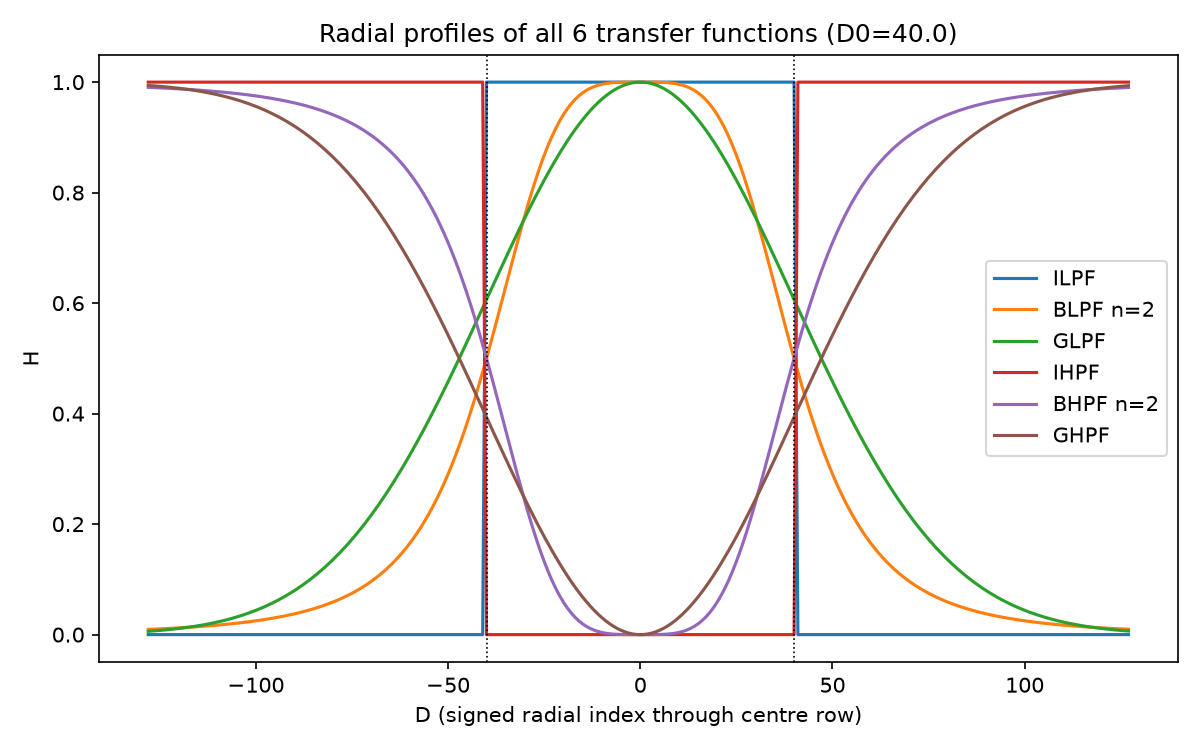
\includegraphics[width=0.8\linewidth]{results/2_1_transfer_functions.png}
\caption{Radial profiles of all six transfer functions (ILPF/BLPF/GLPF, low- and high-pass) at
$D_0=40$: the ILPF's hard wall, BLPF's intermediate roll-off, and GLPF's smoothest roll-off are
clearly visible.}
\label{fig:transfer-functions}
\end{figure}

\subsection{Energy-based cutoff selection (\S2.1b)}

\begin{table}[H]
\centering
\begin{tabular}{@{}lr@{}}
\toprule
$\alpha$ & radius $r$ (padded spectrum) \\
\midrule
90\%   & 15.30 \\
95\%   & 45.54 \\
99\%   & 409.04 \\
99.5\% & 558.74 \\
\bottomrule
\end{tabular}
\caption{Power-retention radii on the characters test pattern's padded spectrum. The large jump
between 95\% ($r\approx45$) and 99\% ($r\approx409$) was confirmed to persist (same qualitative
jump) on the unpadded spectrum as well, ruling it out as a padding artifact.}
\label{tab:energy}
\end{table}

\subsection{Inverse design problem (\S2.1c)}

Given $H(D{=}10)=16/17$ and $H(D{=}40)=1/17$: dividing the two Butterworth equations eliminates
$D_0$, giving $(40/10)^{2n}=256=4^4$, so $2n=4\Rightarrow n=2$. Substituting back,
$(10/D_0)^4=1/16\Rightarrow D_0=20$. Verified with \texttt{make\_filter}:
$H(D{\approx}10)=0.941176$ and $H(D{\approx}40)=0.058824$, exactly matching $16/17$ and $1/17$.
For the smallest integer order attenuating to $\le1\%$ at $D=2D_0$: need $2^{2n}\ge99$; $2^6=64<99$
fails ($n=3$), $2^8=256\ge99$ succeeds, so the \textbf{smallest order is $n=4$}.

\subsection{Ringing prediction and measurement (\S2.2)}

\begin{table}[H]
\centering
\begin{tabular}{@{}rrrrr@{}}
\toprule
$D_0$ & measured OS (\%) & predicted OS (\%) & measured peak dist.\ (px) & predicted peak dist.\ (px) \\
\midrule
10 & 3.44  & 8.95 & 50 & 51.2 \\
20 & 11.45 & 8.95 & 26 & 25.6 \\
40 & 8.27  & 8.95 & 12 & 12.8 \\
80 & 8.78  & 8.95 & 6  & 6.4  \\
\bottomrule
\end{tabular}
\caption{ILPF step-edge overshoot and first-peak distance: measured vs.\ predicted, for
$D_0\in\{10,20,40,80\}$ on the $P=1024$ padded grid.}
\label{tab:ringing-ilpf}
\end{table}

Peak distance matches the prediction closely at every $D_0$. Overshoot matches closely for
$D_0=40,80$ but deviates for $D_0=10,20$: the closed-form prediction assumes a purely 1-D
band-limiting filter, exact only for an infinite straight edge, whereas the square has finite
extent (256 px) in $y$ too, giving its true 2-D spectrum a narrow sinc-shaped spread around $v=0$.
The 2-D disk-shaped ideal filter clips this spread asymmetrically when $D_0$ is comparable to the
spread's lobe spacing ($D_0=10,20$); once $D_0$ is safely larger, the disk behaves like a pure 1-D
band and the match is close. The Gaussian LPF's predicted zero overshoot (non-negative, sum-to-one
spatial kernel) was confirmed exactly: measured overshoot is $0.0000\%$ at every $D_0\in
\{10,20,40,80\}$.

\begin{table}[H]
\centering
\begin{tabular}{@{}rrr@{}}
\toprule
$n$ & measured overshoot (\%) & $|\min h|/\max h$ \\
\midrule
1  & $\approx0.00$ ($9.3\times10^{-6}$) & $\approx0.00$ ($2.5\times10^{-6}$) \\
2  & 3.36 & 0.0432 \\
3  & 5.60 & 0.0966 \\
5  & 7.50 & 0.1577 \\
10 & 8.49 & 0.1999 \\
20 & 8.43 & 0.2124 \\
\bottomrule
\end{tabular}
\caption{Butterworth order sweep at fixed $D_0=40$: overshoot and the 1-D kernel ratio
$|\min h|/\max h$ both increase monotonically with order, approaching the ideal-filter limit
($\approx8.95\%$) as $n\to\infty$.}
\label{tab:butterworth-order}
\end{table}

The $n=1$ kernel is non-negative to numerical precision (ratio $\approx0$), which by the
non-negative-kernel proof (\S2.6) guarantees no overshoot; higher orders develop increasingly deep
negative side-lobes, producing ringing that grows with the ratio.

\begin{figure}[H]
\centering
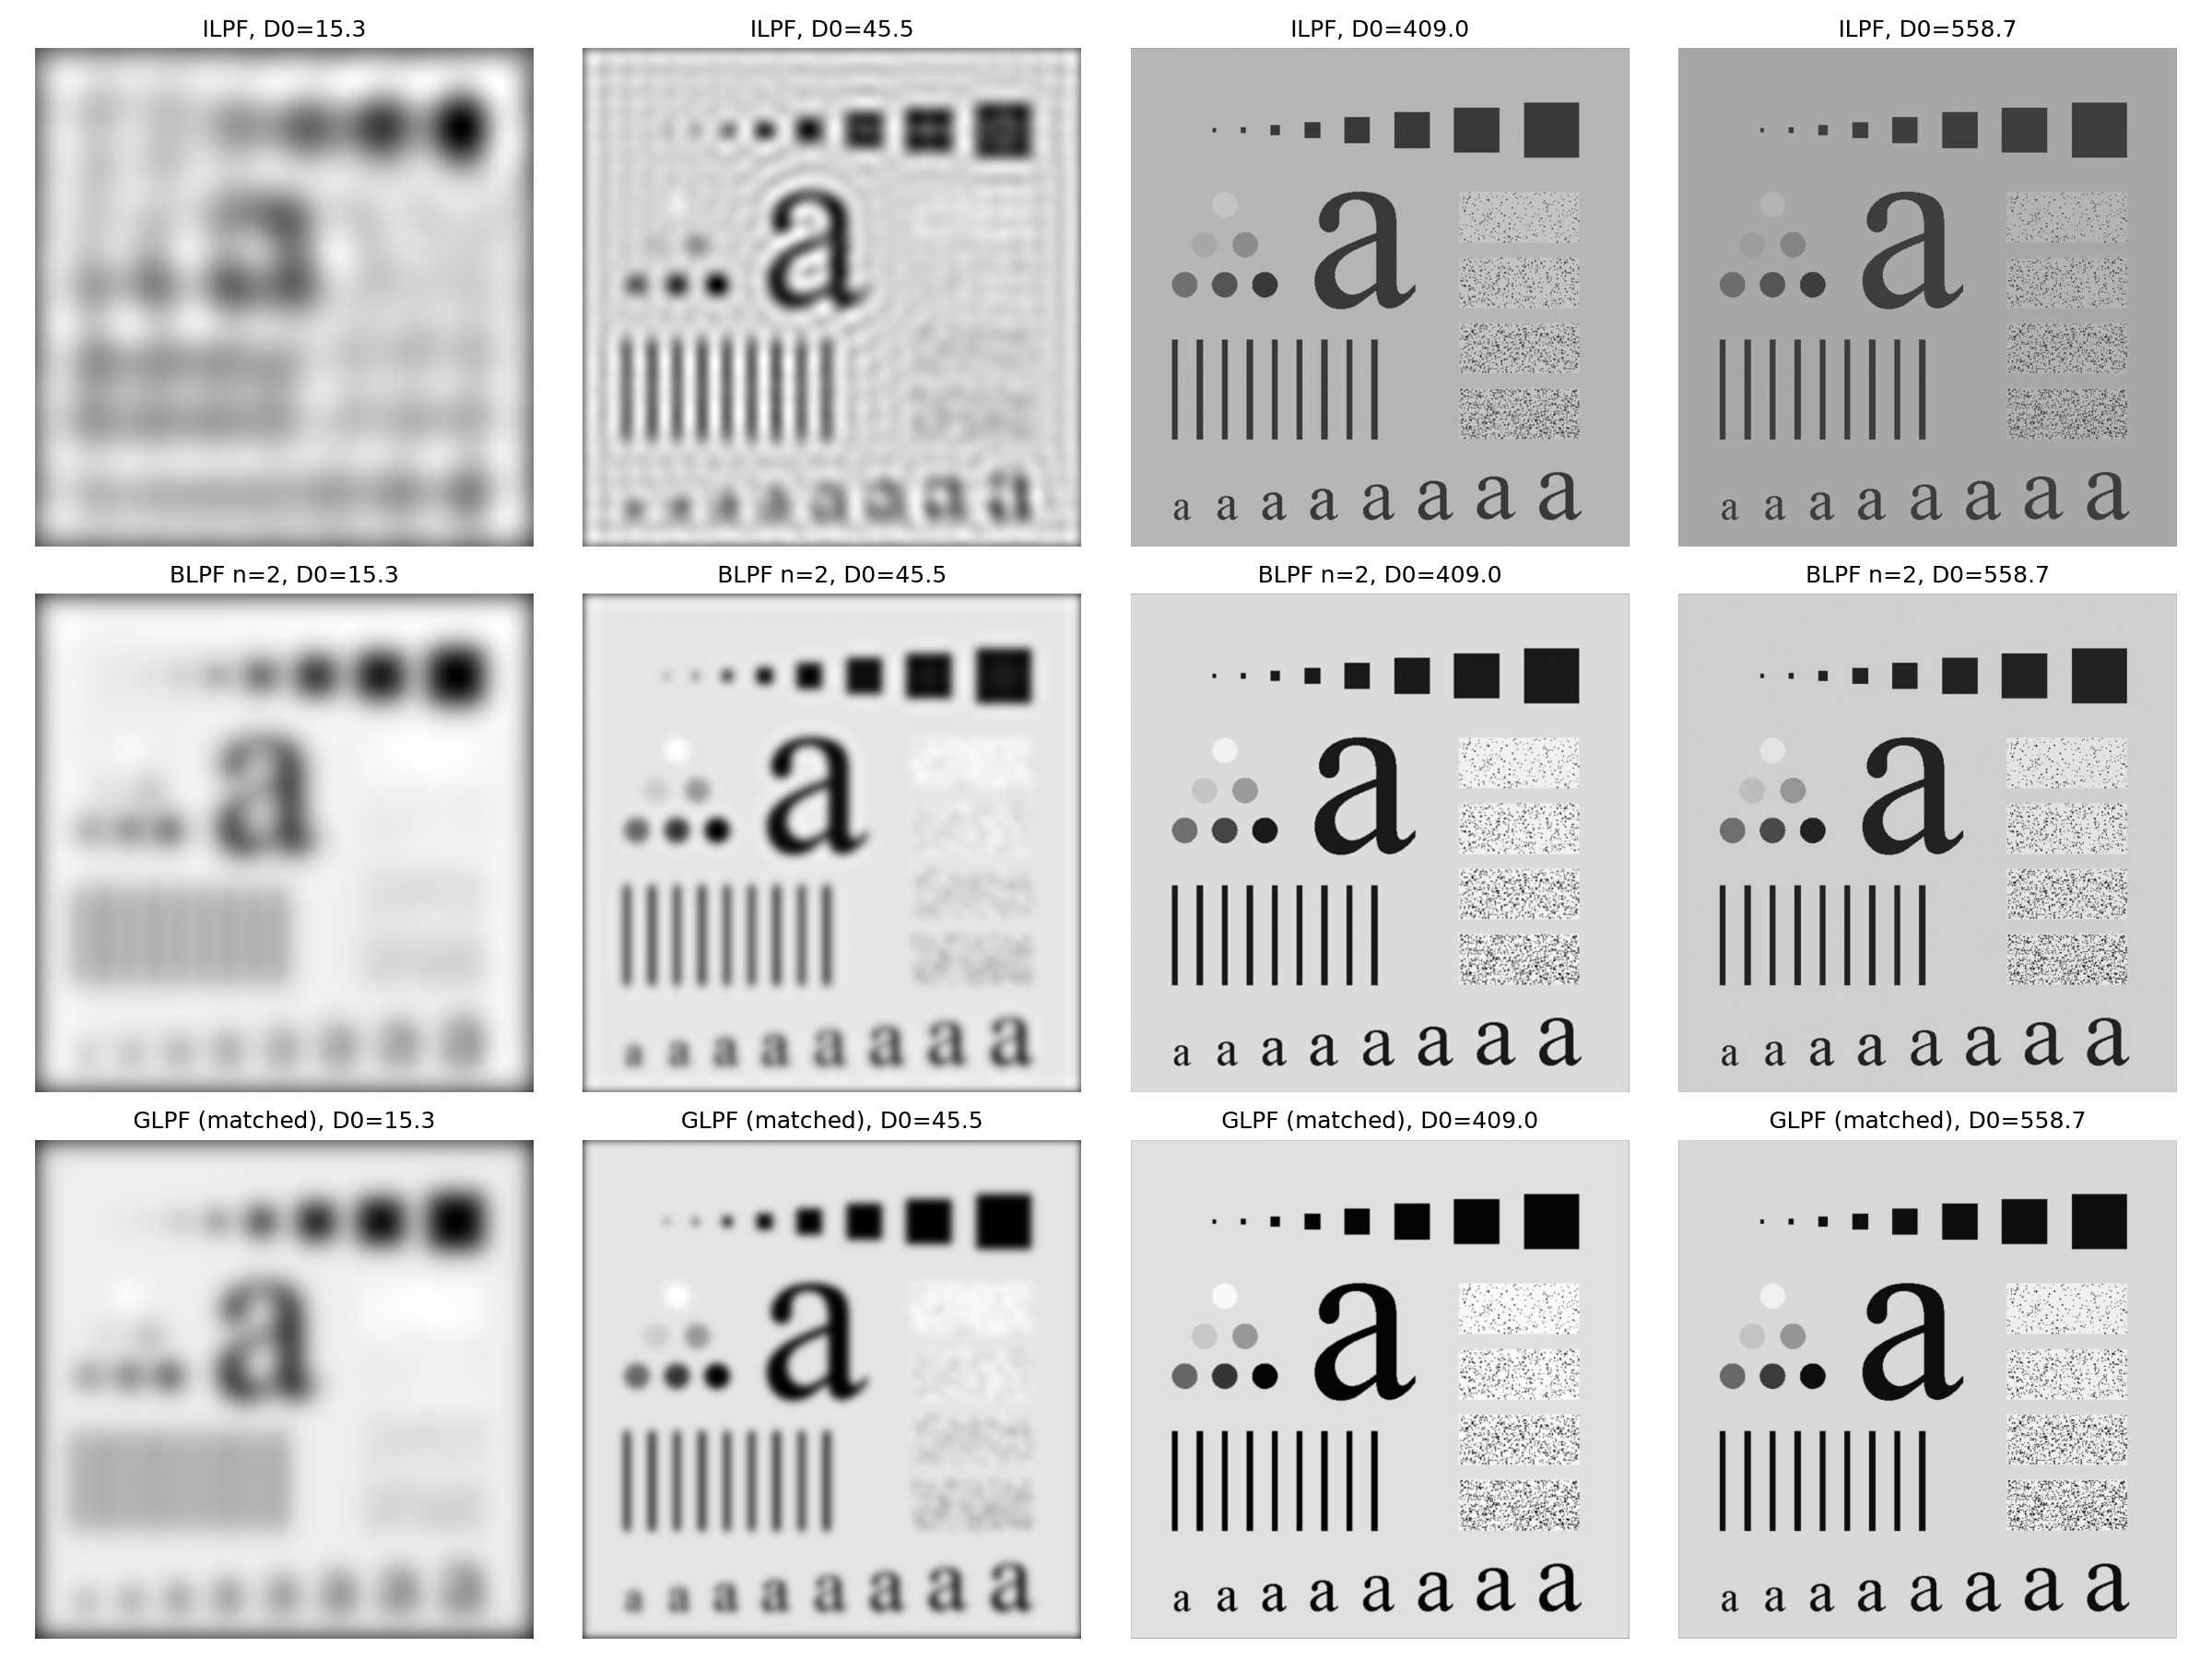
\includegraphics[width=0.8\linewidth]{results/2_2c_visual_grid.png}
\caption{ILPF, BLPF ($n=2$), and GLPF (matched $D_0'$) applied to the characters test pattern at
the four \S2.1b power-retention radii. Ringing (faint periodic bands) is clearly visible around the
``a'' and the squares in the ILPF row at $D_0\approx45.5$ and is essentially absent from the BLPF
and GLPF rows at the same cutoff.}
\label{fig:visual-grid}
\end{figure}

\begin{table}[H]
\centering
\begin{tabular}{@{}rrr@{}}
\toprule
$D_0$ & $\sigma_s$ (px) & $\max|g_{\text{freq}}-g_{\text{spatial}}|$ \\
\midrule
10  & 21.900 & 0.0157 \\
40  & 5.475  & 0.0177 \\
160 & 1.369  & 0.0186 \\
\bottomrule
\end{tabular}
\caption{Gaussian equivalence check: $\sigma_s=P/(2\pi D_0)$ predicts the matching spatial-domain
kernel, verified against \texttt{scipy.ndimage.gaussian\_filter}. All errors are $\le0.019$
intensity levels out of 0--255 ($<0.01\%$), confirming the derivation; the small nonzero residual
and its slight growth with $D_0$ arise from differing discretization/truncation choices between the
frequency-domain filter (sampled on an integer index grid, inverted via a circular, zero-padded
DFT) and \texttt{scipy.ndimage.gaussian\_filter} (a finite-support, truncated-at-$4\sigma$ kernel
with zero boundary handling).}
\label{tab:gaussian-equiv}
\end{table}

\subsection{Applications (\S2.3)}

\begin{table}[H]
\centering
\begin{tabular}{@{}lrr@{}}
\toprule
Family & best $D_0$ in $[5,150]$ & peak PSNR (dB) \\
\midrule
Ideal              & 150 & 27.46 \\
Butterworth ($n=2$) & 150 & 28.72 \\
Gaussian           & 150 & 29.20 \\
\bottomrule
\end{tabular}
\caption{PSNR vs.\ $D_0$ sweep on noisy \texttt{cameraman.tif} ($\sigma=20$, seed 7), mandated
range $D_0\in[5,150]$. Within this range PSNR is still rising at $D_0=150$ for all three families;
the ordering Gaussian $\ge$ Butterworth $\ge$ Ideal holds throughout.}
\label{tab:psnr-sweep}
\end{table}

\begin{figure}[H]
\centering
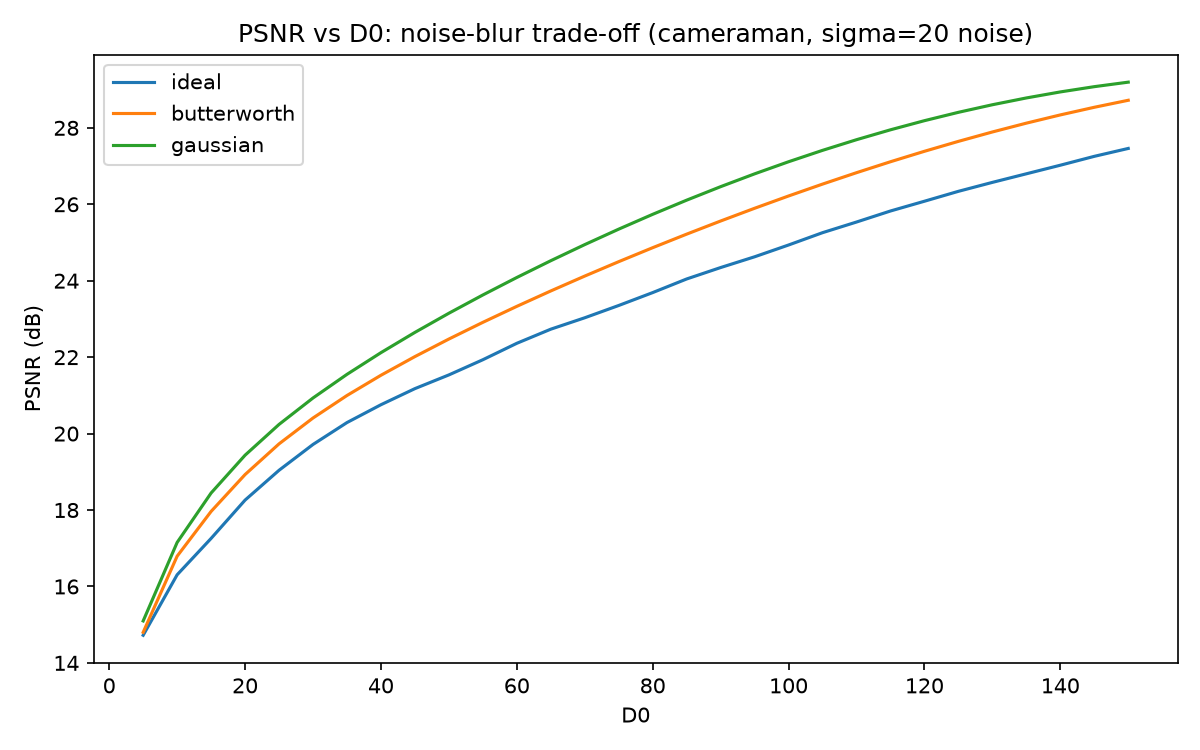
\includegraphics[width=0.8\linewidth]{results/2_3a_psnr_sweep.png}
\caption{PSNR vs.\ $D_0$ for ideal, Butterworth, and Gaussian low-pass denoising of noisy
\texttt{cameraman.tif}. The Gaussian and Butterworth curves dominate the ideal filter's curve at
every $D_0$ tested, consistent with their gradual roll-off already attenuating noise power
approaching the cutoff rather than passing it at full strength up to a hard wall.}
\label{fig:psnr-sweep}
\end{figure}

\begin{figure}[H]
\centering
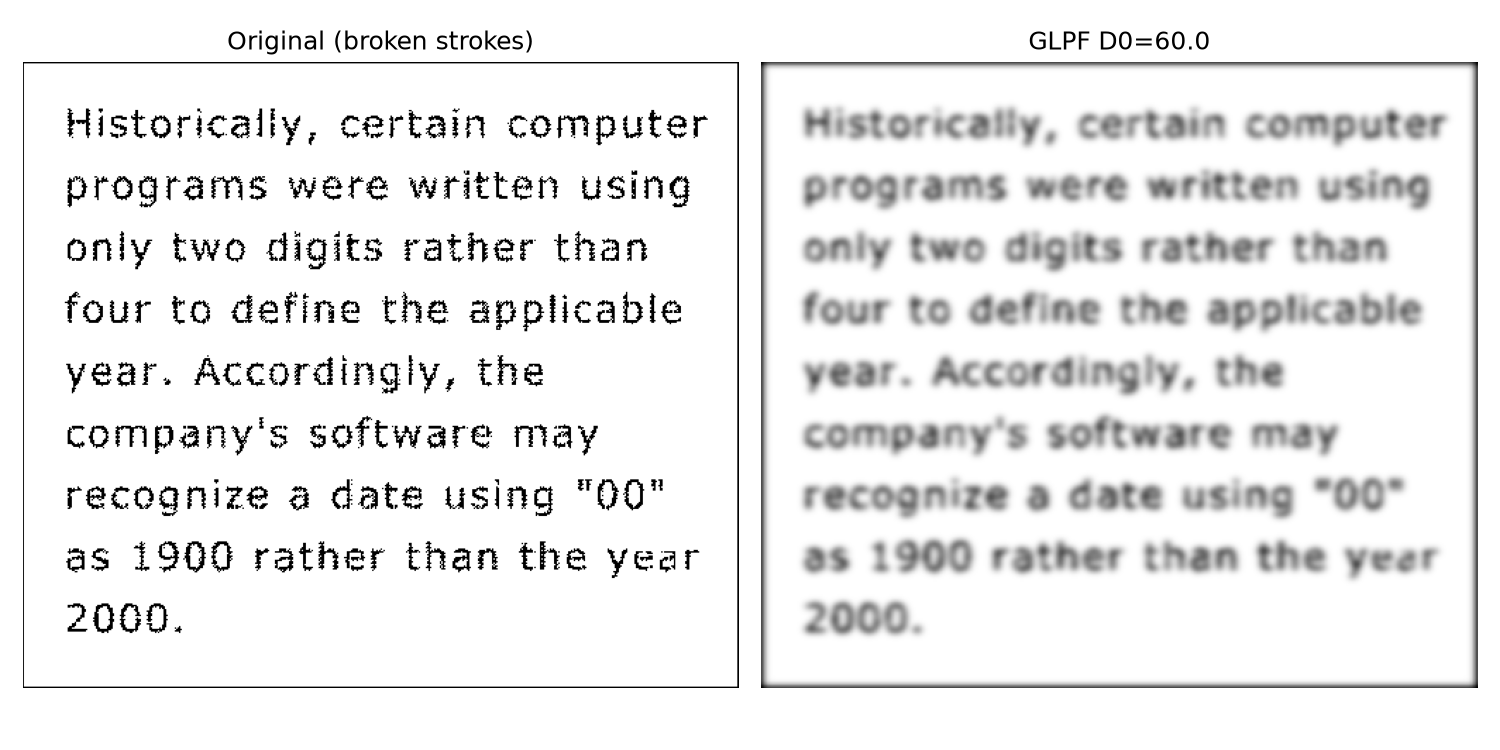
\includegraphics[width=0.8\linewidth]{results/2_3b_character_repair.png}
\caption{\texttt{text\_gaps.tif} before and after Gaussian low-pass filtering at $D_0=60$: the
1--2-pixel gaps in broken strokes are bridged while the characters remain legible, with no ringing
artifacts (unlike an ideal filter at the same half-amplitude radius would be expected to produce).}
\label{fig:character-repair}
\end{figure}

\begin{table}[H]
\centering
\begin{tabular}{@{}lr@{}}
\toprule
Filter & output mean \\
\midrule
IHPF & 2.26 \\
BHPF & 2.33 \\
GHPF & 3.29 \\
\bottomrule
\end{tabular}
\caption{Mean intensity of IHPF/BHPF/GHPF outputs on \texttt{thumb\_print.tif} at a common
half-amplitude radius $D_0=30$. All three are small because $H_{\text{HP}}(P/2,P/2)=1-H_{\text{LP}}(0)=0$
at the exact DC bin, so the full padded canvas's mean is always removed by construction (the
cropped sub-block need not itself average to exactly zero, hence the small nonzero residuals).}
\label{tab:highpass-means}
\end{table}

\begin{figure}[H]
\centering
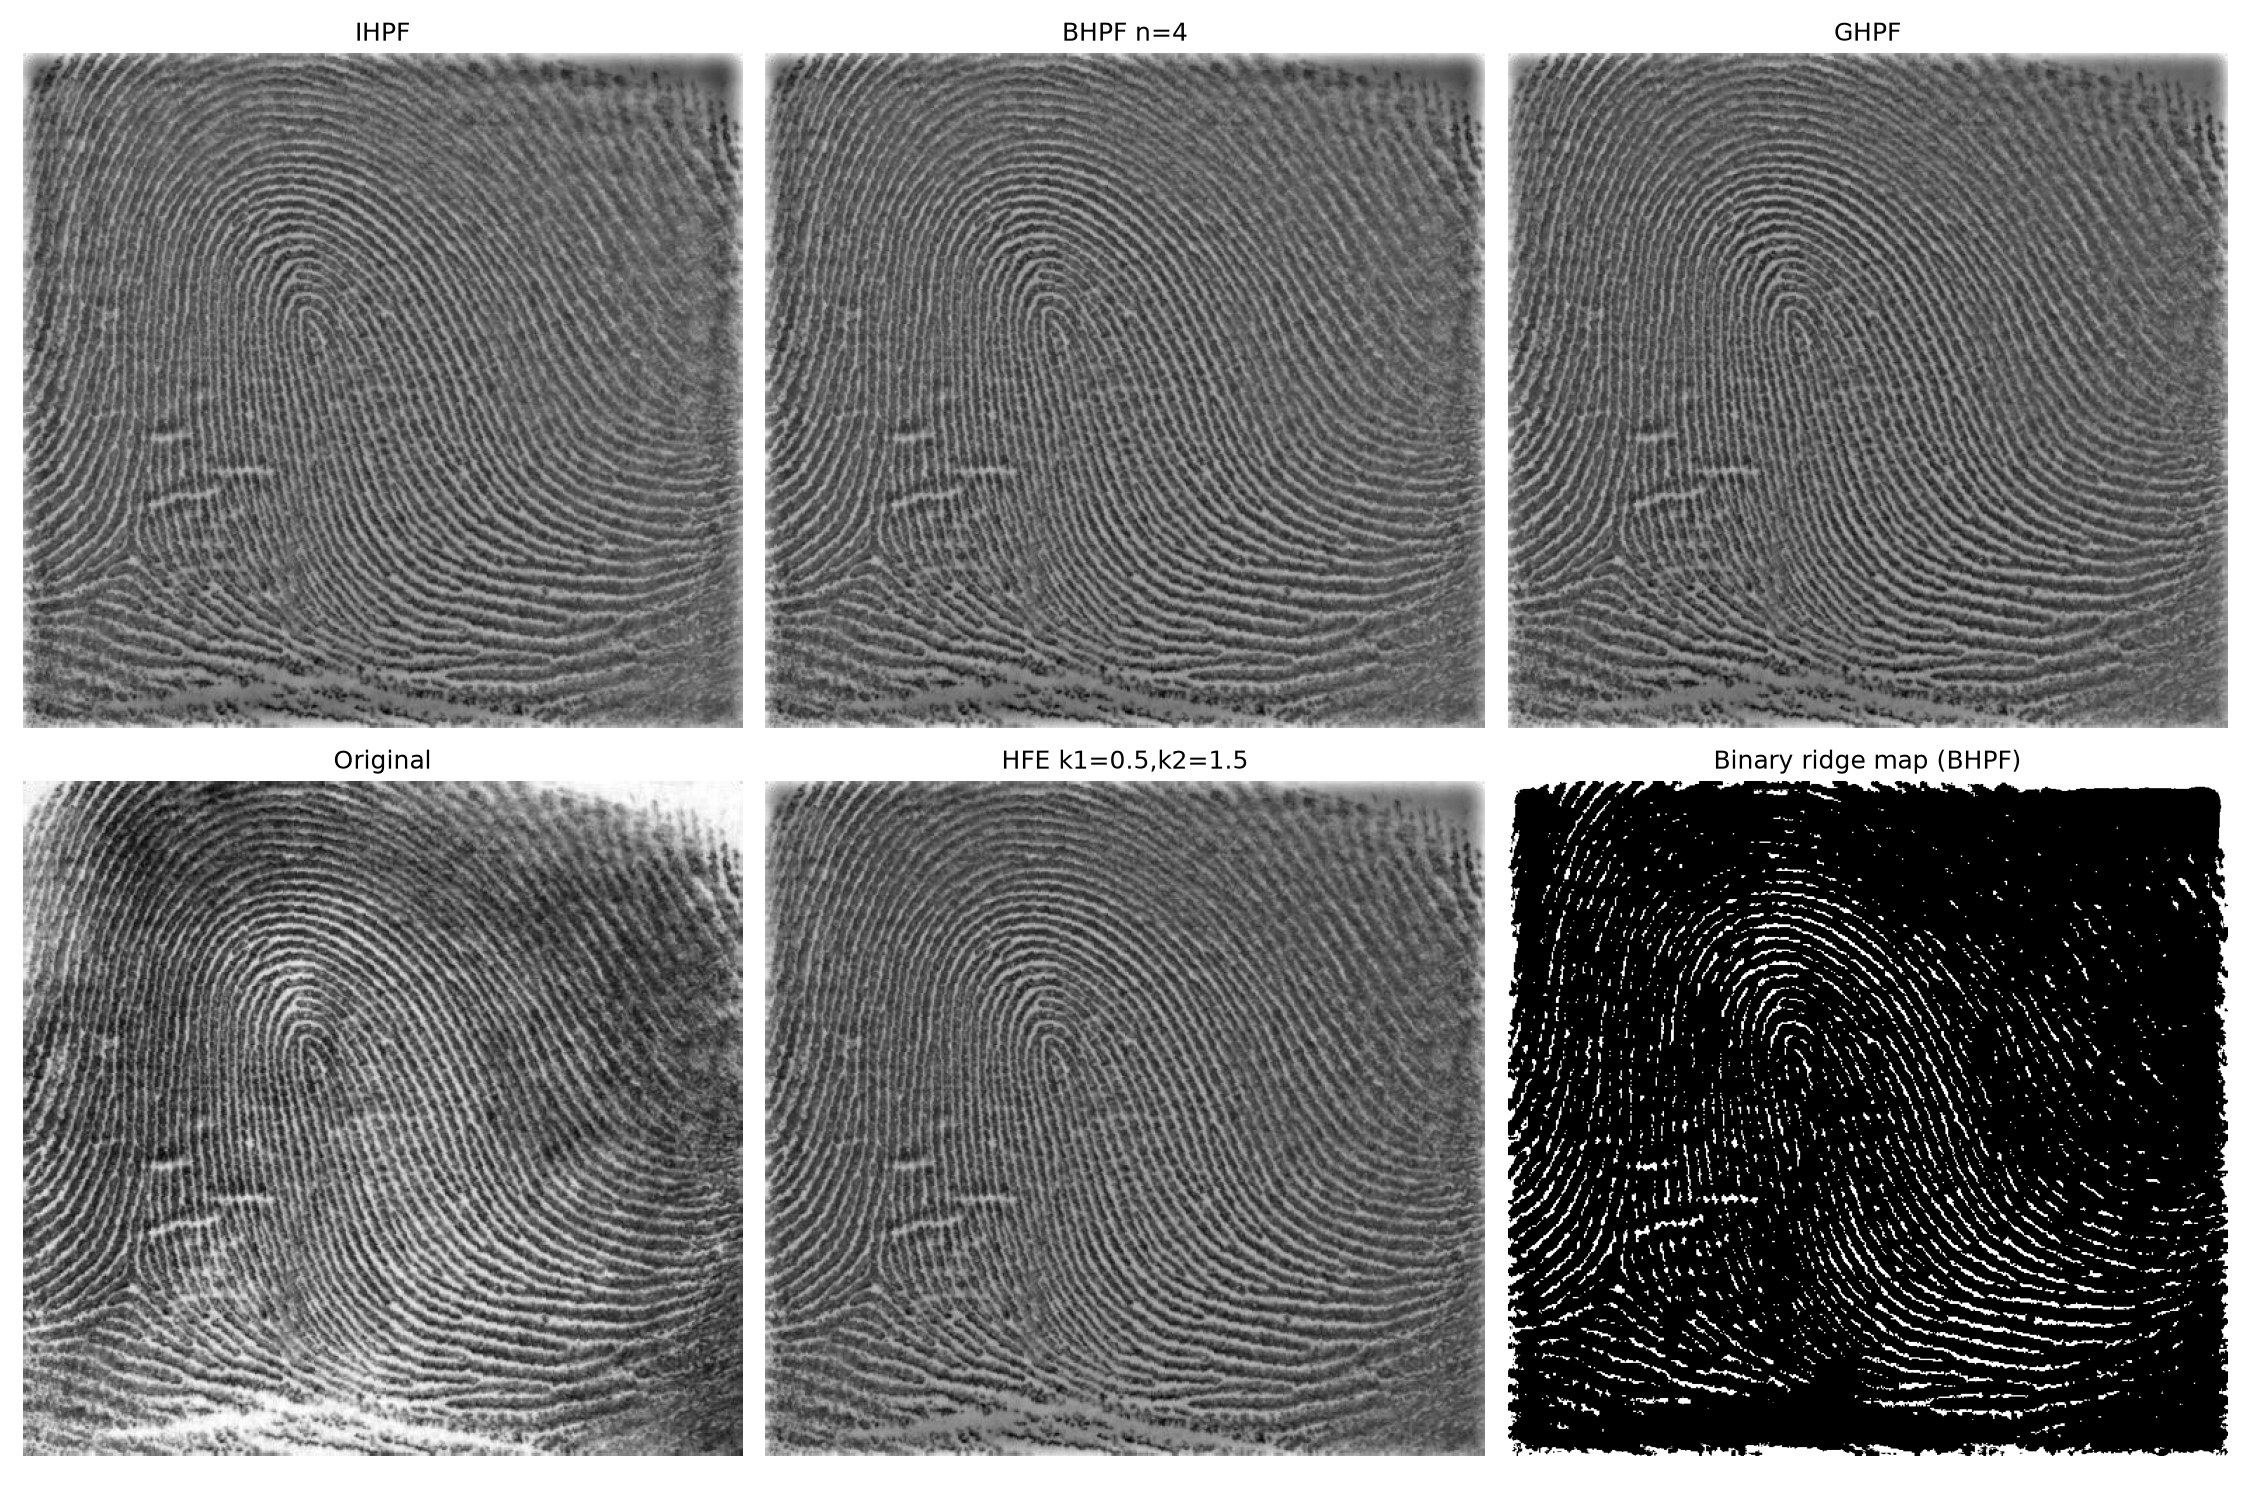
\includegraphics[width=0.8\linewidth]{results/2_3c_highpass.png}
\caption{Top row: IHPF/BHPF($n{=}4$)/GHPF applied to \texttt{thumb\_print.tif}, flat and
near-featureless as expected from the removed DC term. Bottom row: high-frequency emphasis
($H_{\text{HFE}}=k_1+k_2H_{\text{HP}}$, $k_1{=}0.5,k_2{=}1.5$) restores tonal shading while keeping
ridges sharpened; and a binary ridge map obtained by thresholding the BHPF output at its 90th
percentile, which is traceable but noisy since a single global threshold is not locally adaptive.}
\label{fig:highpass}
\end{figure}

\section{Conclusion}

A single \texttt{make\_filter} implementation, built directly from the ideal/Butterworth/Gaussian
formulas, was validated analytically and numerically, and used throughout a consistent
zero-pad--centre--multiply--invert--crop pipeline. The cutoff-matching derivation showed that a
shared numerical $D_0$ does not give a like-for-like comparison across filter families, and the
matched Gaussian parameter $D_0'=D_0/\sqrt{2\ln2}$ was used in every subsequent comparison. The
energy-based cutoff analysis showed that spectral power concentrates heavily near DC without that
implying the remaining high frequencies are visually unimportant, and an inverse-design problem was
solved exactly and verified numerically ($n=2$, $D_0=20$). The ringing study confirmed, both by a
dated pre-implementation closed-form Gibbs-phenomenon prediction and by direct measurement, that
the ideal filter produces a cutoff-independent $\approx8.95\%$ step-edge overshoot while the
Gaussian filter produces none, with the Butterworth family interpolating between the two as its
order increases and its spatial kernel develops deeper negative side-lobes --- exactly as proven by
the non-negative-kernel argument. The $\sigma_s=P/(2\pi D_0)$ derivation was confirmed against an
independent spatial-domain Gaussian implementation to within 0.02 intensity levels. Finally, the
denoising, text-repair, and fingerprint high-pass/high-frequency-emphasis applications demonstrated
the practical consequence of these transfer-function shapes: smoother roll-offs (Gaussian,
Butterworth) consistently outperform the ideal filter on both quantitative (PSNR) and qualitative
(ringing-free repair, clean sharpening) grounds, establishing the sharpness/ringing trade-off as the
central practical lesson of frequency-domain filtering.

\end{document}
